\section{Objectives}

Following handout PDF pages 85--87, compare direct clocks, two-inverter clock restoration, skew in a three-stage dynamic-DFF register, and low-frequency retention.

\section{Handout requirements and test mapping}

\begin{center}
\small
\setlength{\tabcolsep}{4pt}
\begin{tabular}{p{.42\linewidth}p{.29\linewidth}p{.18\linewidth}}
\toprule
Requirement & Deck prefix and conditions & Status \\
\midrule
Step 1: slower clock edges and higher frequency & 01; direct, 9 pairs & Measured \\
Step 2: repeat with two inverter stages & 01; buffered, same pairs & Measured \\
Step 3: three DFFs; third clock leads/lags & 02; 9 signed skews & Measured \\
Keep source rise/fall at 0.2 ns & 02; fixed source slew & Preserved \\
Q1: low-frequency storage; Q2/3: buffer/race & 03; 10 us, 25/115 C & Measured and analyzed \\
\bottomrule
\end{tabular}
\end{center}

\section{Circuit and timing derivation}

The direct case uses an ideal complementary voltage. The buffered case uses the first and second inverter outputs as complementary phases, including real delay, nonsimultaneous transitions, and loading. In the three-stage chain, stages 1 and 2 share one buffered clock; stage 3 receives an independently shifted raw pulse followed by an identical two-inverter chain. Positive skew means that the third clock is later.

With destination-clock delay $s$, common constraints are $t_{CQ,\max}+t_{PD,\max}+t_{SU}\leq T+s$ and $t_{CQ,\min}+t_{CD,\min}\geq t_H+s$. Positive skew can relax setup while worsening hold. A buffer can restore edge slope without guaranteeing race immunity.

\section{Simulation setup and interpretation}

The supplied encrypted MOS model is evaluated at a baseline supply of 1.0 V and 25\,$^\circ$C. The 1.0 V value is a teaching condition, not a verified voltage rating. These results do not reproduce the handout's original process or supply conditions. Unless stated in the deck, $W_n/W_p/L=0.6/1.8/0.25\,\mu\mathrm m$, bulks are tied to their corresponding rails, and output load is 5 fF. Transmission-gate and weak-feedback dimensions are specified explicitly in each deck.

PrimeSim HSPICE S-2021.09 win64 was used with \texttt{RUNLVL=6}, \texttt{ACCURATE}, and \texttt{WARNLIMIT=100}. Every baseline and \texttt{.alter} analysis concluded without errors or failed measurements. The simulator still reports suppressed warnings associated with encrypted blocks; this does not establish that the model is warning-free or that those warnings are harmless. The \texttt{.tran} print interval is not a fixed integration step: the solver uses adaptive timesteps. A finite sweep is not a complete process qualification.

Unless stated otherwise, the declared functional diagnostic uses $V\leq0.2$ V for low and $V\geq0.8$ V for high. These are report-level interpretation thresholds, not numerical handout requirements or extracted receiver noise margins. Correct samples do not exclude glitches between samples. Figures are redrawn from actual simulation data; \texttt{results/} contains per-case waveforms, measurements, and derived comparison CSV files.

Public decks omit model loading paths; model configuration is added only to local execution copies. The model itself is not distributed. The first two filename digits identify the deck numbers used below. Every deck is standalone.

\section{Results}

\begin{center}
\small
\setlength{\tabcolsep}{4pt}
\begin{tabular}{lrrr}
\toprule
Period (ns) & Edge (ns) & Direct correct/8 & Buffered correct/8 \\
\midrule
20 & 0.2 & 8 & 8 \\
20 & 1 & 8 & 8 \\
20 & 5 & 8 & 8 \\
10 & 0.2 & 8 & 8 \\
10 & 1 & 8 & 8 \\
10 & 2 & 8 & 8 \\
4 & 0.2 & 8 & 8 \\
4 & 1 & 4 & 4 \\
2 & 0.2 & 8 & 4 \\
\bottomrule
\end{tabular}
\end{center}

Samples occur at $0.49T$, referenced to the raw clock rise beginning at $0.25T$; buffer delay consumes part of the same observation interval. Both versions give only 4/8 correct samples at 4 ns/1 ns. At 2 ns/0.2 ns, direct gives 8/8 and buffered 4/8. This table therefore does not establish that buffering always raises intrinsic maximum frequency. Edge quality, insertion delay, and receiver sampling time must be distinguished.

\begin{figure}[htbp]
\centering
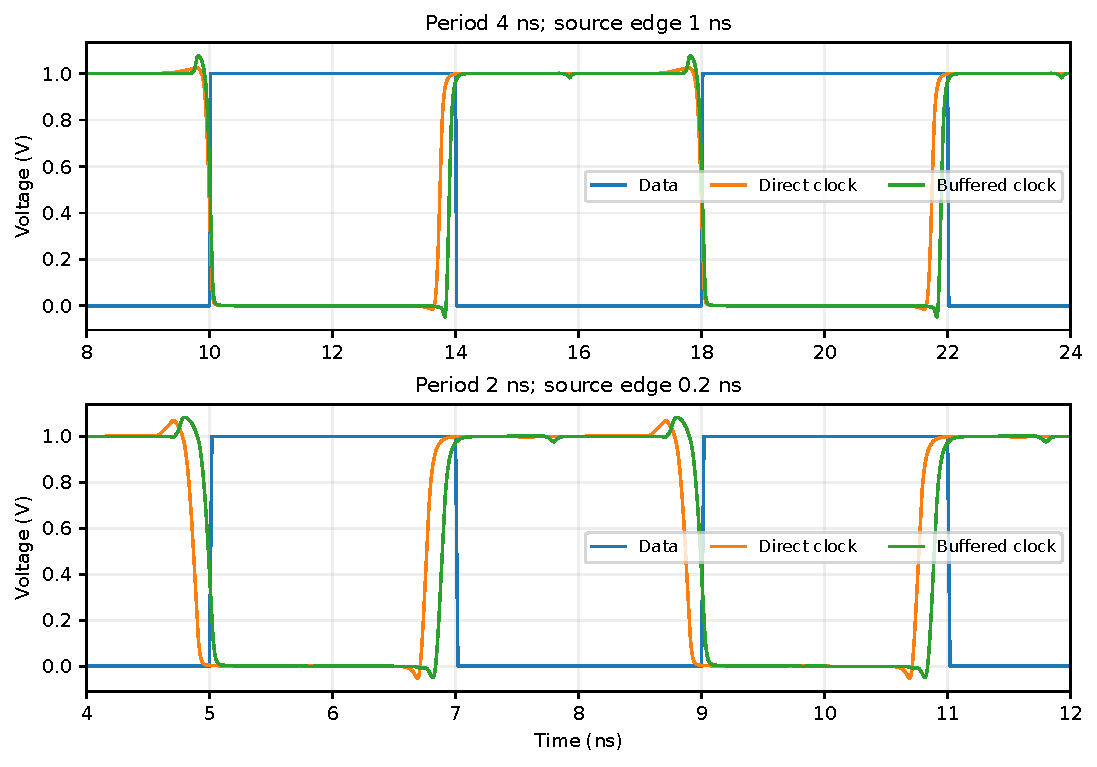
\includegraphics[width=.96\linewidth]{figures/clock_slope.pdf}
\caption{Two cases near the observation deadline; buffer insertion delay affects fixed-time interpretation.}
\end{figure}

\begin{center}
\small
\setlength{\tabcolsep}{4pt}
\begin{tabular}{lrrr}
\toprule
Third-clock skew (ns) & Correct/7 & First sample (V) & Second sample (V) \\
\midrule
0 & 7 & 1.00001 & 0.00000 \\
-0.2 & 7 & 1.00001 & 0.00000 \\
-0.5 & 7 & 1.00001 & 0.00000 \\
-1 & 7 & 1.00001 & 0.00000 \\
-2 & 7 & 1.00001 & 0.00000 \\
0.2 & 7 & 1.00001 & 0.00000 \\
0.5 & 0 & 0.00000 & 1.00000 \\
1 & 0 & 0.00001 & 1.00001 \\
2 & 0 & 0.00000 & 1.00000 \\
\bottomrule
\end{tabular}
\end{center}

Zero through +0.2 ns lag gives 7/7 correct samples. At +0.5 ns and beyond, the sequence becomes the opposite data sequence, giving 0/7, consistent with a late destination clock allowing same-cycle data through a hold/race path. Tested leads from -0.2 to -2 ns give 7/7; this does not imply arbitrary negative skew is safe. The positive boundary is bracketed only by +0.2 and +0.5 ns, without continuous bisection.

\begin{figure}[htbp]
\centering
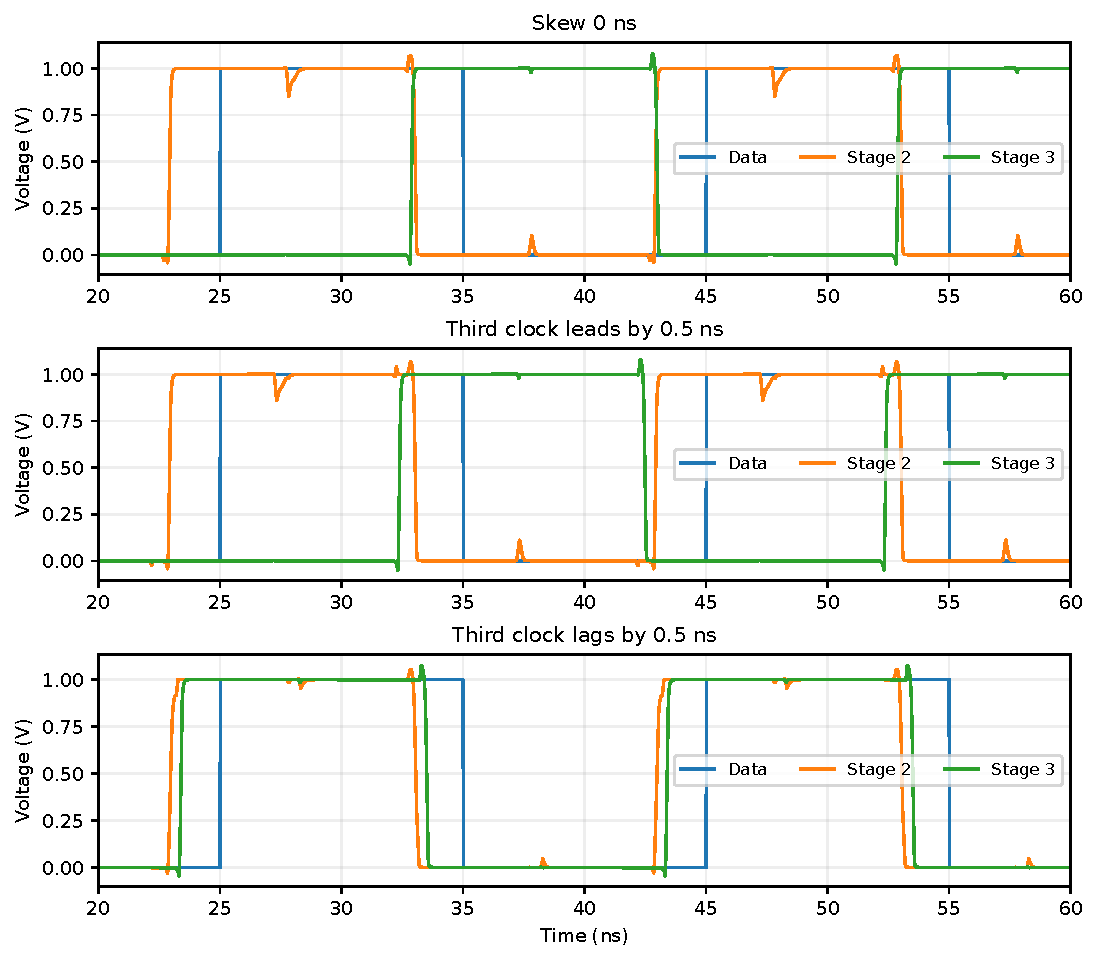
\includegraphics[width=.96\linewidth]{figures/clock_skew.pdf}
\caption{Three-stage data sequences at zero skew and with the third clock leading or lagging.}
\end{figure}

\begin{center}
\small
\setlength{\tabcolsep}{4pt}
\begin{tabular}{lrr}
\toprule
Temp. (C) & Master X at 7 us (V) & Slave Z at 12 us (V) \\
\midrule
25 & 0.582685 & 0.084038 \\
115 & 0.662096 & 0.117369 \\
\bottomrule
\end{tabular}
\end{center}

\begin{figure}[htbp]
\centering
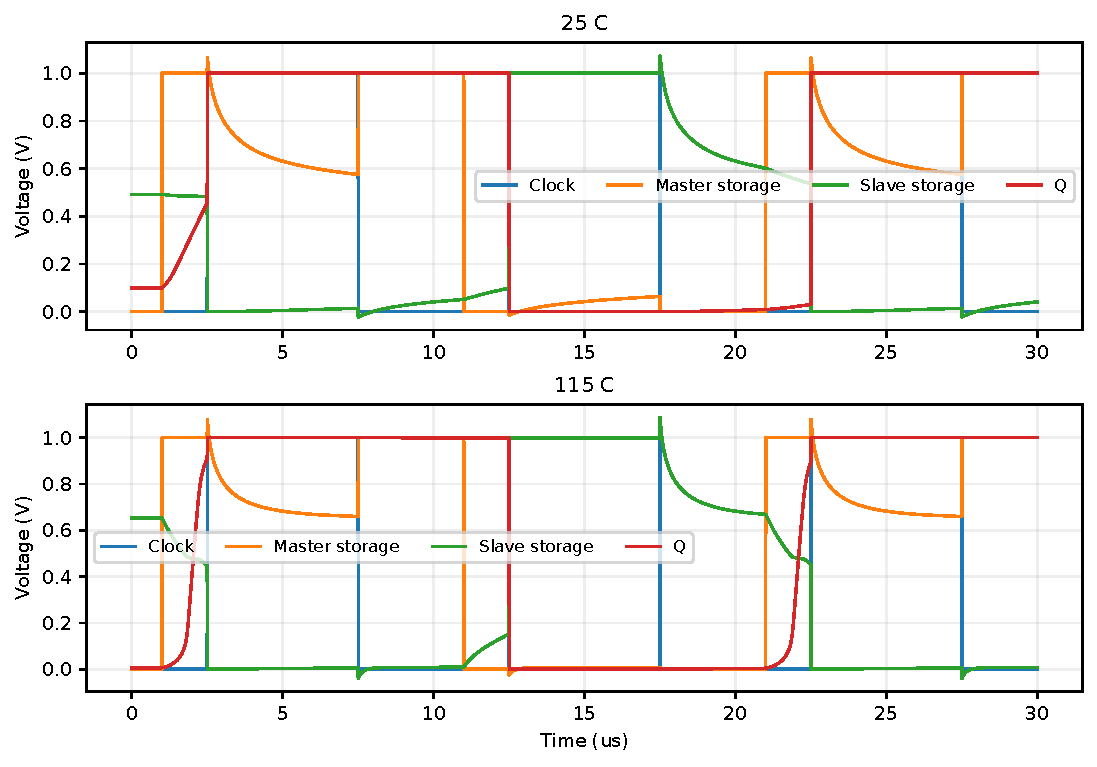
\includegraphics[width=.96\linewidth]{figures/slow_clock.pdf}
\caption{Internal floating storage nodes with a 10 us clock period.}
\end{figure}

\section{Discussion, differences, and unverified scope}

At low frequency, floating storage nodes move away from the rails. Even if selected output samples remain correct, dynamic latches cannot be treated as indefinite storage. The two-temperature results represent net leakage, not isolated junction leakage; monotonic deterioration cannot be imposed on every node. Remedies include static/weak feedback, nonoverlapping phases, clock-tree skew control, and setup/hold compliance. NORA/TSPC changes race conditions but remains subject to analog coupling and data timing. The rewrite adds matched direct/buffer tests, signed skew, and low-frequency internal-node observations, explicitly accounting for the clock buffers' insertion delay.
